\chapter{Python}

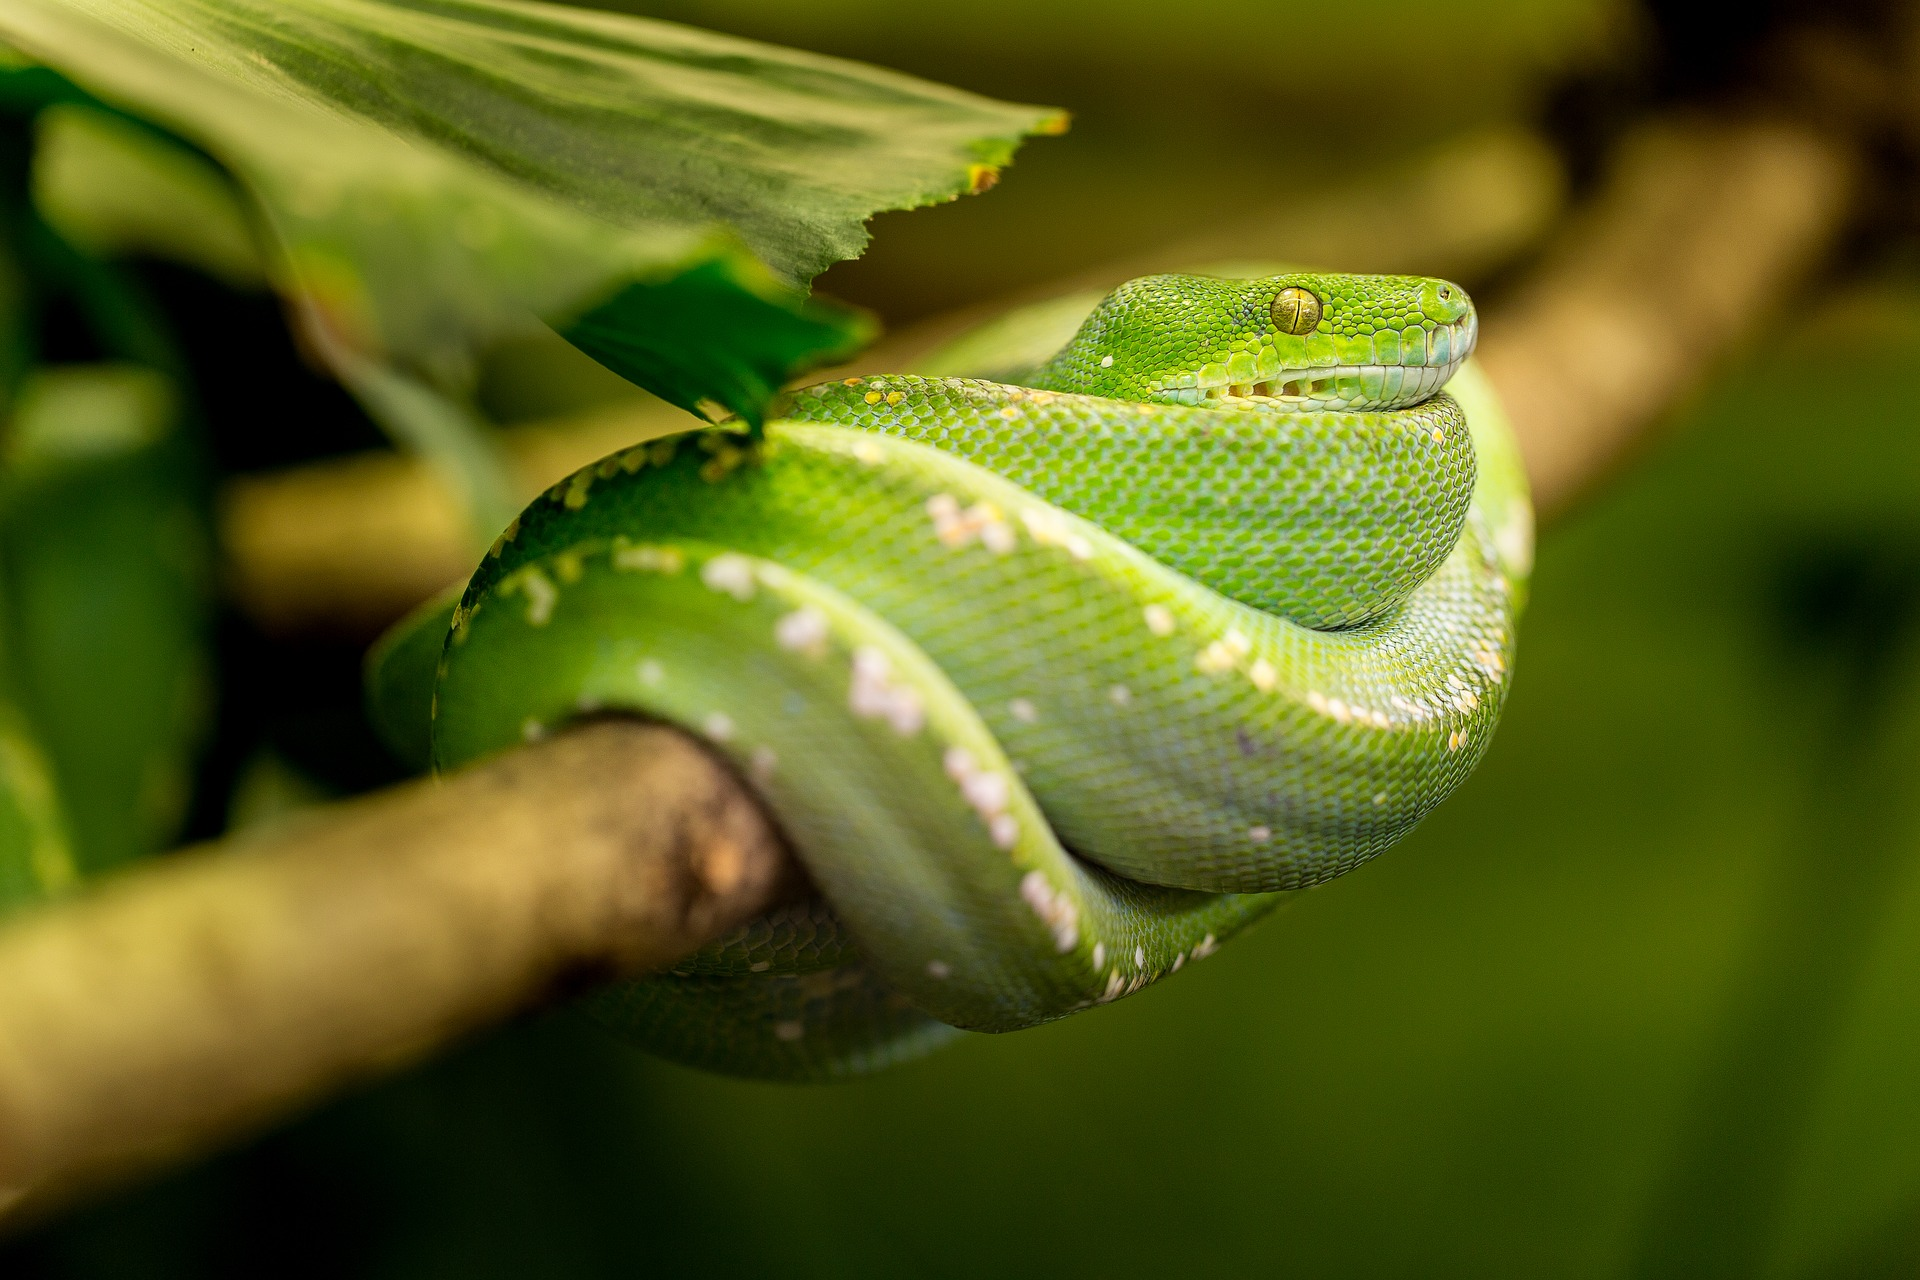
\includegraphics[scale=0.85]{../images/snake-1634293_1920.jpg}

\justify
Getting started in writing programs is easy with Python. It is highly extensible since there are many add on modules available from a collection known as Pypi\footnote{\url{https://pypi.org/}} . Python is
fairly easy to learn, especially when compared to other languages. Python runs "everywhere", for all intents and purposes. For all these reasons, Python is a great choice.

\justify
An item of note, Python3\index{Python3} is our only choice at this point. Python 2.x
End of Life was January 1st, 2020\footnote{\url{https://github.com/python/devguide/pull/344}}.


\section{The \_\_init\_\_.py File}

We add this file to let the Python interpreter know that the directories
it is found in are a contiguous part of our Python project. Since module
imports and function definitions in this file are available to all the
python code files in the directory, we can use it to our advantage. For
example, try adding this quick and dirty logging function to
python/devsecops/lib/\_\_init\_\_.py

\begin{mybox}{\thetcbcounter: python/devsecops/lib/\_\_init\_\_.py}
import logging\\
from pathlib import Path\\

Path("/var/log/devsecops").mkdir(parents=True, exist\_ok=True)\\
logging.basicConfig(\\
   filename="/var/log/devsecops/devsecops.log",\\
   level=logging.DEBUG,\\
   format="[%(asctime)s] [%(filename)s:%(lineno)s - %(funcName)5s() - %(processName)s] %(levelname)s - %(message)s"]
\end{mybox}

Now we can create a Python file log\_test.py and call the logger from
within like so:

\begin{mybox}{\thetcbcounter: log\_test.py}
import logging\\
from pathlib import Path\\

def main():\\
   logging.debug('Loggy Loggerton')\\
   if \_\_name\_\_=="\_\_main\_\_":\\
   main()
\end{mybox}

Check the results in the file /var/log/devsecops/devsecops.log.

\section{Requirements File}

\justify
A requirements file under python/requirements.txt\index{requirements.txt} lists the required
Python modules needed to build and run any Python portions of our
cloudlab project. We also add a check in the Makefile to verify the
existence of the requirements.txt file. The intention is, so we can
quickly cut and paste the Makefile into a new project, but not break
anything if no requirements are present yet.

\section{Test requirements}

\justify
Some requirements are strictly intended to be part of the test harness,
but are not needed for the application proper. Using a separate file,
such as python/requirements-test.txt\index{requirements-test.txt}, makes this delineation clear to
folks who are not familiar with the project.

\justify
Note that we can also include test requirements in our tox.ini file, as detailed in the next section.

\section{Project Testing}

Security and reliability in our lab and rapid prototyping work is just as important as it is in our work for the Production environment. In fact, you might say it's even more important since today's rapid mock ups
can easily wind up making it into the build pipeline when folks are under a time crunch to deliver.

There are many test frameworks out there, lots of great ideas put forth by the community. For our current efforts, we've settled on Tox\index{Tox} as the framework of choice. It dovetails nicely with the rest of our patterns. Tox allows us to manage requirements for virtual environments when testing, acts as a front end to pytest and coverage modules, and much more. It is highly configurable and extensible. For example we can test
that an application is compatible with multiple versions of Python.

\justify
Use the make test command inside the docker container to run the test suite for the project.

\justify
An example tox.ini\index{tox.ini} file follow. Take notice of the "deps" section, where
Python module requirements can be specified. In our current configuration, these are in lieu of test harness requirements specified in our python/requirements-test.txt file.

\begin{mybox}{\thetcbcounter: An example tox.ini file}
[tox]\\
envlist = py38
skip\_missing\_interpreters = true\\

[testenv]\\
setenv =\\
  PYTHONPATH = .\\
  PYTHONHTTPSVERIFY=0\\
deps =\\
  coverage\\
  pytest\\
commands =\\
  coverage run -m pytest -v --capture=sys\\
  coverage report --omit="*/test*,.tox/*"
\end{mybox}

\section{Test Cases}

\justify
Unit and functional testing is foundational in developing robust, secure
code. We want to be sure that when we create new code, we are also
adding test cases to our test suite that fully cover the new classes,
functions, and so on.

single: Test Cases (Python)

\justify
Consider the following example unit test case. The purpose is to test
that the function check\_docker() in the file python/cloudlab/lib/helper\_functions.py returns True when called from inside a Docker container.

\begin{mybox}{\thetcbcounter: An example Unit test case}
import pytest
from cloudlab.lib.helper\_functions import check\_docker


def test\_check\_docker():\\
   assert(check\_docker())\\
\end{mybox}

\hypertarget{test-coverage}{%
\section{Test Coverage}\label{test-coverage}}

As mentioned previously, we can avail ourselves of the coverage module
by adding it to test-requirements.txt or the deps section of our tox.ini
file. The purpose is to automatically generate a report on how much of
our code is "covered" by test cases in python/test.

single: Coverage single: Test Coverage

\section{Python Directory Structure}

Files and folders relevant to the Python portions of our project are
shown in the diagram below.

\begin{description}
\item[digraph folders \{]
1 {[}label="python", shape=folder{]}; 2 {[}label="devsecops",
shape=folder{]}; 3 {[}label="lib", shape=folder{]}; 4
{[}label="requirements.txt", shape=rectangle{]}; 5
{[}label="requirements-test.txt", shape=rectangle{]}; 6
{[}label="\_\_init\_\_.py", shape=rectangle{]}; 7
{[}label="\_\_init\_\_.py", shape=rectangle{]}; 8 {[}label="test",
shape=folder{]}; 9 {[}label="devsecops.py", shape=rectangle{]}; A
{[}label="\_\_init\_\_.py", shape=rectangle{]}; B
{[}label="\_\_init\_\_.py", shape=rectangle{]}; C {[}label="tox.ini",
shape=rectangle{]}; D {[}label="helper\_functions.py",
shape=rectangle{]};

1 -\textgreater{} 2; 1 -\textgreater{} 6; 2 -\textgreater{} 3; 1
-\textgreater{} 4; 1 -\textgreater{} 5; 2 -\textgreater{} 7; 1
-\textgreater{} 8; 2 -\textgreater{} 9; 8 -\textgreater{} A; 3
-\textgreater{} B; 1 -\textgreater{} C; 3 -\textgreater{} D;
\end{description}

\}
